
%(BEGIN_QUESTION)
% Copyright 2011, Tony R. Kuphaldt, released under the Creative Commons Attribution License (v 1.0)
% This means you may do almost anything with this work of mine, so long as you give me proper credit

Suppose an instrument technician connects an oscilloscope to a FOUNDATION Fieldbus segment as shown with the intention of viewing the signal:

$$\includegraphics[width=15.5cm]{i00890x01.eps}$$

Explain what is wrong with this setup, and what problems it might cause in the segment.  Correspondingly, how {\it should} the oscilloscope be connected to the segment cable?

\vskip 20pt \vbox{\hrule \hbox{\strut \vrule{} {\bf Suggestions for Socratic discussion} \vrule} \hrule}

\begin{itemize}
\item{} Explain how this improper use of an oscilloscope could even pose a {\it safety} hazard to the technician if used on a different kind of circuit (something other than a Fieldbus H1 segment).
\item{} An all-too-common practice to overcome this problem involves powering the oscilloscope through an {\it isolation transformer} so that it's AC supply is ungrounded.  Explain how this solution overcomes the measurement problem seen in the diagram, and also explain why this practice can be unsafe.
\end{itemize}

\underbar{file i00890}
%(END_QUESTION)





%(BEGIN_ANSWER)

Connecting a line-powered oscilloscope to a FF segment in this manner creates a {\it ground fault} in the system, which could (at worst) shut down communication throughout the entire segment!

%(END_ANSWER)





%(BEGIN_NOTES)

The oscilloscope should be configured for {\it differential} measurement, where two input channels are used, and no ground clips are connected to any point of the FF segment.

%INDEX% Electronics review: oscilloscope usage
%INDEX% Fieldbus, FOUNDATION (H1): segment troubleshooting

%(END_NOTES)

